% %% file: template.tex = LaTeX template for article-like report 
%% init: sometime 1993
%% last: Feb  8 2015  Rob Rutten  Deil
%% site: http://www.staff.science.uu.nl/~rutte101/rrweb/rjr-edu/manuals/student-report/

%% First read ``latex-bibtex-simple-manual.txt'' at
%% http://www.staff.science.uu.nl/~rutte101/Report_recipe.html

%% Start your report production by copying this file into your XXXX.tex.
%% Small changes to the header part will make it an A&A or ApJ manuscript.

%%%%%%%%%%%%%%%%%%%%%%%%%%%%%%%%%%%%%%%%%%%%%%%%%%%%%%%%%%%%%%%%%%%%%%%%%%%%
\documentclass{aa}   %% Astronomy & Astrophysics style class
%\documentclass[a4paper,10pt]{report}
\usepackage{graphicx,url,twoopt}
%\usepackage{biblatex}
\usepackage{enumitem}
\usepackage{amsmath}
\usepackage[varg]{txfonts}           %% A&A font choice
%\usepackage{hyperref}                %% for pdflatex
%%\usepackage[breaklinks]{hyperref}  %% for latex+dvips
%%\usepackage{breakurl}              %% for latex+dvips
%\usepackage{pdfcomment}              %% for popup acronym meanings
%\usepackage{acronym}                 %% for popup acronym meanings
\usepackage{calrsfs}
\DeclareMathAlphabet{\pazocal}{OMS}{zplm}{m}{n}

\usepackage{natbib}
% \hypersetup{
%   colorlinks=true,   %% links colored instead of frames
%   urlcolor=blue,     %% external hyperlinks
%   linkcolor=red,     %% internal latex links (eg Fig)
% }

 %\bibpunct{(}{)}{;}{a}{}{,}    %% natbib cite format used by A&A and ApJ
 
 \pagestyle{plain}   %% undo the fancy A&A pagestyle 

%% Add commands to add a note or link to a reference
\makeatletter
\newcommand{\bibnote}[2]{\@namedef{#1note}{#2}}
\newcommand{\biblink}[2]{\@namedef{#1link}{#2}}
\makeatother

%% Commands to make citations ADS clickers and to add such also to refs
%% May 2014: they give error stops ("Illegal parameter number ..."}
%%   for plain latex with TeX Live 2013; the ad-hoc fixes added below let
%%   latex continue instead of stop within these commands.
%%   Please let me know if you know a better fix!
%%   No such problem when using pdflatex.
\makeatletter
 \newcommandtwoopt{\citeads}[3][][]{%
   \nonstopmode%              %% fix to not stop at error message in latex
   \href{http://adsabs.harvard.edu/abs/#3}%
        {\def\hyper@linkstart##1##2{}%
         \let\hyper@linkend\@empty\citealp[#1][#2]{#3}}%   %% Rutten, 2000
   \biblink{#3}{\href{http://adsabs.harvard.edu/abs/#3}{ADS}}%
   \errorstopmode}            %% fix to resume stopping at error messages 
 \newcommandtwoopt{\citepads}[3][][]{%
   \nonstopmode%              %% fix to not stop at error message in latex
   \href{http://adsabs.harvard.edu/abs/#3}%
        {\def\hyper@linkstart##1##2{}%
         \let\hyper@linkend\@empty\citep[#1][#2]{#3}}%     %% (Rutten 2000)
   \biblink{#3}{\href{http://adsabs.harvard.edu/abs/#3}{ADS}}%
   \errorstopmode}            %% fix to resume stopping at error messages
 \newcommandtwoopt{\citetads}[3][][]{%
   \nonstopmode%              %% fix to not stop at error message in latex
   \href{http://adsabs.harvard.edu/abs/#3}%
        {\def\hyper@linkstart##1##2{}%
         \let\hyper@linkend\@empty\citet[#1][#2]{#3}}%     %% Rutten (2000)
   \biblink{#3}{\href{http://adsabs.harvard.edu/abs/#3}{ADS}}%
   \errorstopmode}            %% fix to resume stopping at error messages 
 \newcommandtwoopt{\citeyearads}[3][][]{%
   \nonstopmode%              %% fix to not stop at error message in latex
   \href{http://adsabs.harvard.edu/abs/#3}%
        {\def\hyper@linkstart##1##2{}%
         \let\hyper@linkend\@empty\citeyear[#1][#2]{#3}}%  %% 2000
   \biblink{#3}{\href{http://adsabs.harvard.edu/abs/#3}{ADS}}%
   \errorstopmode}            %% fix to resume stopping at error messages 
\makeatother

%%%%%%%%%%%%%%%%%%%%%%%%%%%%%%%%%%%%%%%%%%%%%%%%%%%%%%%%%%%%%%%%%%%%%%%%%%%%
\begin{document}  

%% simple header.  Change into A&A or ApJ commands for those journals

\twocolumn[{%
\vspace*{4ex}

\begin{center}
  {\Large \bf The recombination history of the universe}\\[4ex]
  {\large \bf Andreas Ellewsen$^1$}\\[4ex]
  \begin{minipage}[t]{15cm}
        $^1$ Institute of Theoretical Astrophysics, University of Oslo, P.O. Box 1029 Blindern, N-0315 Oslo, Norway\\
             
        
    {\bf Abstract.} I set up the background cosmology of the universe.
    
  \vspace*{2ex}
  \end{minipage}
\end{center}
}]

%%%%%%%%%%%%%%%%%%%%%%%%%%%%%%%%%%%%%%%%%%%%%%%%%%%%%%%%%%%%%%%%%%%%%%%%%%%%
\section{Introduction}\label{sec:introduction}
%%%%%%%%%%%%%%%%%%%%%%%%%%%%%%%%%%%%%%%%%%%%%%%%%%%%%%%%%%%%%%%%%%%%%%%%%%%%
In this project I will follow the algorithm presented in Callin (2005)[1] for simulating the cosmic microwave background.  
This is part two of four for this project.

In the first part I set up the background cosmology of the universe. 
In this part the goal is to compute the optical depth $\tau$ as a function of $x$, where $x$ is the logarithm of the scale factor $a$. And the visibility function $g$, and its scaled version $\tilde{g} = g/\pazocal{H}$. We also want the first and second derivatives of both of these functions with respect to $x$.

As in the first part of the project I will continue building on the skeleton code provided.

%%%%%%%%%%%%%%%%%%%%%%%%%%%%%%%%%%%%%%%%%%%%%%%%%%%%%%%%%%%%%%%%%%%%%%%%%%%%
\section{Equations}\label{sec:Equations}
%%%%%%%%%%%%%%%%%%%%%%%%%%%%%%%%%%%%%%%%%%%%%%%%%%%%%%%%%%%%%%%%%%%%%%%%%%%%
The optical depth is defined
\begin{equation}\label{tau}
 \tau(\eta) = \int_\eta^{\eta_0}n_e\sigma_T ad\eta'.
\end{equation}
This is the probability for a photon to scatter between some previous time $\eta$ and today $\eta_0$. This way, if one at time $\eta$ had a beam of photons with intensity $I_0$ one would today at time $\eta_0$ have a beam with intensity $I = I_0exp(-\tau(\eta))$.
Looking at equation \ref{tau}, $n_e$ is the electron density, $\sigma_T$ the Thompson cross-section, and $a$ the scale factor.

Equation \ref{tau} can be rewritten on differential form as
\begin{equation}\label{tau2}
 \frac{d\tau}{d\eta}  = \dot{\tau}= - n_e\sigma_T a.
\end{equation}
Or since we generally use $x$ instead of $\eta$, as
\begin{equation}
 \frac{d\tau}{dx} = \tau' = -\frac{n_e\sigma_T a}{\pazocal{H}}.
\end{equation}
The Thompson cross section is
\begin{equation}
 \sigma_T =  \frac{8\pi\alpha^2}{3m_e^2} = 6.652462\times10^{-29} \textmd{m}^2.
\end{equation}


The only unknown quantity left in equation \ref{tau2} is $n_e$. 
Before finding a way to compute this quantity we define the visibility function as
\begin{equation}
 g(\eta) = -\dot{\tau}e^{-\tau(\eta)} = \pazocal{H}\tau'e^{-\tau(x)} = g(x)
\end{equation}
\begin{equation}
 \tilde{g}(x) \equiv -\tau'e^{-\tau}=\frac{g(x)}{\pazocal{H}(x)}. 
\end{equation}
This visibility function is normalized as
\begin{equation}
 \int_0^{\eta_0} g(\eta)d\eta = \int_{-\infty}^0 \tilde{g}(x)dx = 1,
\end{equation}
and thus it can be interpreted as a probability distribution. The visibility function then gives the probability that a CMB photon was last scattered at conformal time $\eta$.

From this we see that if we want to find the visibility function $g$, we will need the optical depth $\tau$ and its derivative, and to find that we need the electron density $n_e$.

To find this we will make some assumptions.
We define 
\begin{equation}
 X_e \equiv \frac{n_e}{n_H} = \frac{n_e}{n_b}.
\end{equation}
Note here that we assume that the number density of baryons is equal to the number density of hydrogen. And thus we have ignored all elements above hydrogen. We also ignore the small difference in mass between neutral hydrogen and free protons. Thus we have
\begin{equation}
 n_H = n_b \simeq \frac{\rho_b}{m_H} = \frac{\Omega_b \rho_c}{m_H a^3}
\end{equation}

The only thing left to find now is $X_e$. There are two equations to choose from when calculating this.
One is the Saha equation, which is valid for $X_e \approx 1$. And the other is Peeble's equation which is valid for all values of $X_e$. 

Saha's equation is
\begin{equation}
 \frac{X_e^2}{1-X_e} = \frac{1}{n_b}\bigg(\frac{m_e k_b T_b}{2\pi \hbar^2}\bigg)^{3/2}e^{-\epsilon_0/k_b T_b},
\end{equation}
where $m_e$ is the electron mass, $k_b$ the Boltzmann constant, $T_b$ the baryon temperature, $\hbar$ the reduced Planck constant, and $\epsilon_0$ the ionization energy of hydrogen. This is a regular quadratic equation which can be solved using the regular method.

Peeble's equation is 
\begin{equation}
\frac{dX_e}{dx} = \frac{C_r(T_b)}{H} \left[\beta(T_b)(1-X_e) - n_H
  \alpha^{(2)}(T_b)X_e^2\right],
\end{equation}
where
\begin{align}
C_r(T_b) &= \frac{\Lambda_{2s\rightarrow1s} +	
  \Lambda_{\alpha}}{\Lambda_{2s\rightarrow1s} + \Lambda_{\alpha} +
  \beta^{(2)}(T_b)}, \\  
\Lambda_{2s\rightarrow1s} &= 8.227 \textrm{s}^{-1}\\
\Lambda_{\alpha} &= H\frac{(3\epsilon_0 c/\hbar)^3}{(8\pi)^2 n_{1s}}\\
n_{1s} &= (1-X_e)n_H \\
\beta^{(2)}(T_b) &= \beta(T_b) e^{3\epsilon_0/4k_b T_b} \\
\beta(T_b) &= \alpha^{(2)}(T_b) \left(\frac{m_e k_b T_b}{2\pi\hbar^2}
\right)^{3/2} e^{-\epsilon_0/k_b T_b} \\
\alpha^{(2)}(T_b) &= \frac{64\pi}{\sqrt{27\pi}}
\frac{\hbar^2 \alpha^2}{c m_e^2}\sqrt{\frac{\epsilon_0}{k_b T_b}}\phi_2(T_b)\\
\phi_2(T_b) &= 0.448\ln(\epsilon_0/k_B T_b).
\end{align}
Here $\alpha$ is the fine structure constant.

At early times $X_e$ should be very close to 1, so we will start with Saha's equation. We define the point where we switch from Saha to Peeble's equation at $X_e = 0.99$. 

With this it should be possible to calculate the electron density, optical depth, and the visibility function.
How this is done is explained in the next section.

%%%%%%%%%%%%%%%%%%%%%%%%%%%%%%%%%%%%%%%%%%%%%%%%%%%%%%%%%%%%%%%%%%%%%%%%%%%%
\section{Implementation}\label{sec:Imp}
%%%%%%%%%%%%%%%%%%%%%%%%%%%%%%%%%%%%%%%%%%%%%%%%%%%%%%%%%%%%%%%%%%%%%%%%%%%%
As in part one of the project we will continue using Fortran90.
We will also be using most of the variables we defined in that part again.
The only thing I want to change is the length of my $x$ array. 
Since the evolution of the optical depth should change fairly little except for around recombination, I set it up with three intervals with different step lengths. The first part goes from $x = -10.5$ to the x value corresponding to redshift $z= 1630.4$ with 300 points. The next goes from the end of the first to $z = 614.2$ with 300 points. And the last one goes from there until today at $z = 0$ with 300 points. This ensures that we have a much better resolution around recombination than the rest.

The next step is to calculate the electron density. The first part of this is easy. One writes in the equations and solves the Saha equation with simple algebra. When the switch to Peebles occurs we make use of the ODE solver used in part one of the project. 


CONTINUE FROM HERE CONTINUE FROM HERE CONTINUE FROM HERE CONTINUE FROM HERE CONTINUE FROM HERE CONTINUE FROM HERE CONTINUE FROM HERE CONTINUE FROM HERE CONTINUE FROM HERE CONTINUE FROM HERE CONTINUE FROM HERE CONTINUE FROM HERE CONTINUE FROM HERE CONTINUE FROM HERE CONTINUE FROM HERE CONTINUE FROM HERE CONTINUE FROM HERE CONTINUE FROM HERE CONTINUE FROM HERE CONTINUE FROM HERE CONTINUE FROM HERE CONTINUE FROM HERE 

We then set the first $x$ value to correspond to $a= 10^{-10}$, and the last to $a=0$ (today). 
I've chosen to use 1000 points for these arrays and make the steps equal in the $x$ array. After that one computes the $a$, and $z$ values for each of the points in this $x$ array. Because of this we now have linear steps in $x$.
With that done, one computes $H$, $\pazocal{H}$, $\rho_x$, and $\Omega_x$ for each $x$ value.

The last thing to find is $\eta(x)$. 
To do this we need to use an ODE solver on equation \ref{eta}. For this we must have some initial value for the function. 
The equation we then want to solve is 
\begin{equation}
 \eta(a) = \int_0^a \frac{da'}{a'\pazocal{H}(a')}
\end{equation}

This can be found by considering that $a\pazocal{H} \rightarrow  H_0\sqrt{\Omega_r+\Omega_\nu}$ as $a \rightarrow 0$. This gives 
\begin{equation}
 \eta(a) = \frac{a}{H_0\sqrt{\Omega_r+\Omega_\nu}}
\end{equation}
for small $a$. And thus one has an initial value.

Plugging this into the ODE solver returns $\eta(x)$ for all values in the $x$ array. Thus completing all calculations needed for the first part of the project. The ODE solver uses the Bulirsch–Stoer algorithm. The step length is set to be one hundredth the length between two neighboring $x$ values.

As preparation for the next part I also spline the resulting $\eta(x)$ values. These are then integrated and evaluated for a new set of $x$ values not equal to but inside the $x$ values used to make the spline. I have over plotted this in the plot for $\eta(x)$ and the functions overlap. 

%%%%%%%%%%%%%%%%%%%%%%%%%%%%%%%%%%%%%%%%%%%%%%%%%%%%%%%%%%%%%%%%%%%%%%%%%%%%
\section{Results}\label{sec:simulate_analytic}
%%%%%%%%%%%%%%%%%%%%%%%%%%%%%%%%%%%%%%%%%%%%%%%%%%%%%%%%%%%%%%%%%%%%%%%%%%%%

$X_e$

  \begin{figure}[ht]
   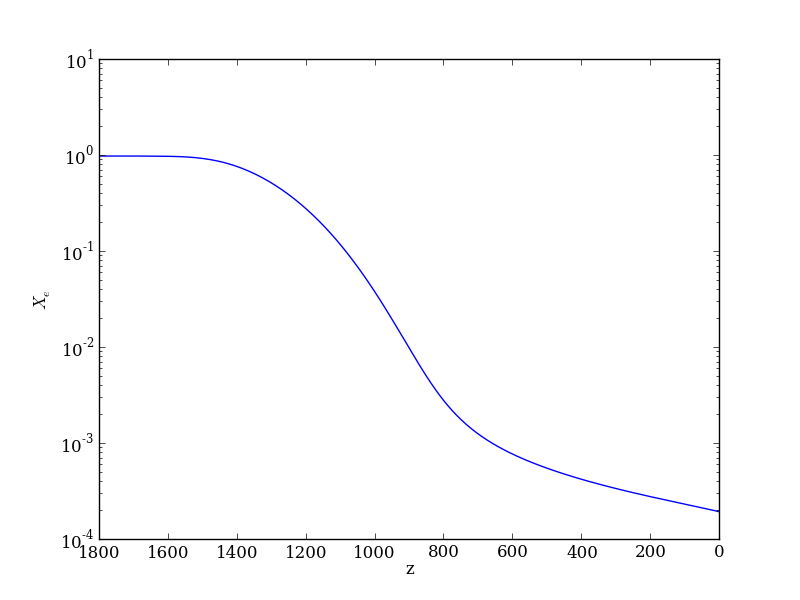
\includegraphics[width=.49\textwidth]{X_e.png}
   \caption{}
  \label{figure0}
  \end{figure}

 
   \begin{figure}[ht]
   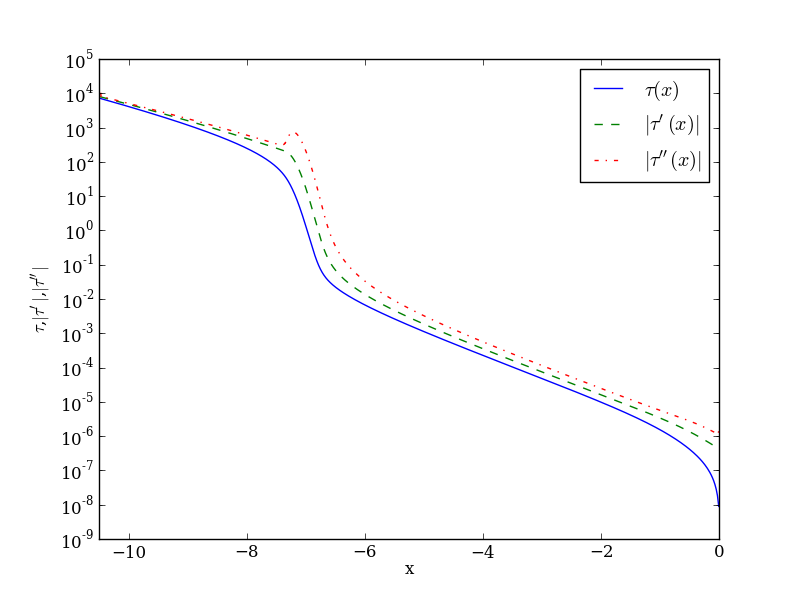
\includegraphics[width=.49\textwidth]{tau.png}
   \caption{}
  \label{figure1}
  \end{figure}
 
 
   \begin{figure}[ht]
   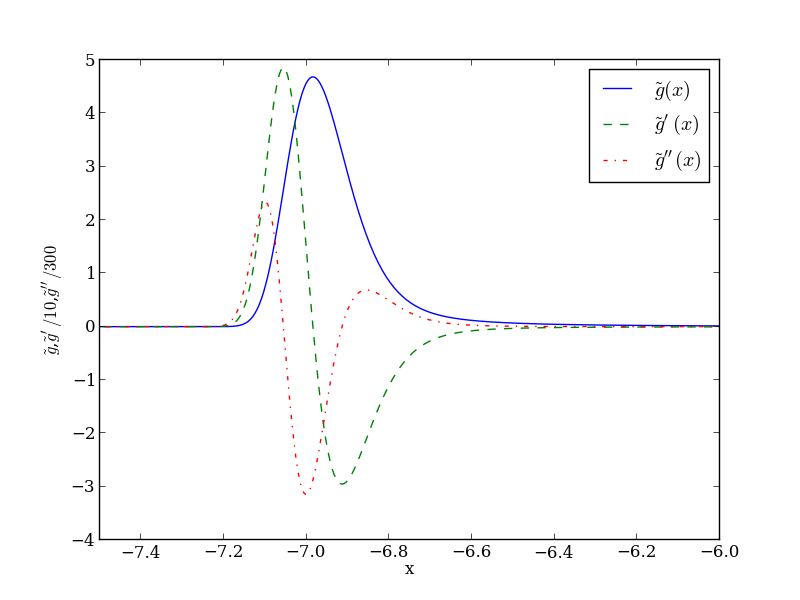
\includegraphics[width=.49\textwidth]{g.png}
   \caption{}
  \label{figure2}
  \end{figure}
%  
%  \begin{figure}[ht]
%   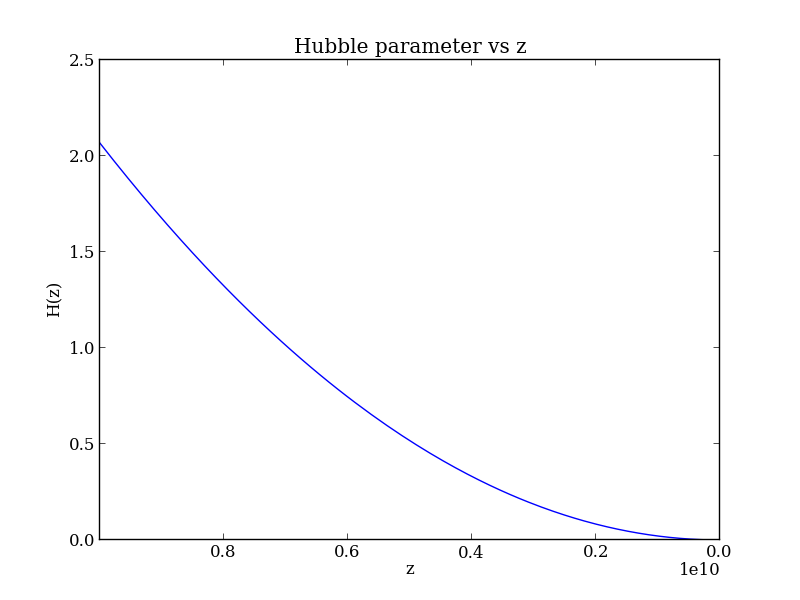
\includegraphics[width=.49\textwidth]{figure_3.png}
%   \caption{The figure depcits the Hubble parameter as a function of redshift $z$. Note that $z$ increases to the left, such that time goes towards the right.}
%  \label{figure3}
%  \end{figure}
% 
% \begin{table}
%  \begin{tabular}{|c|c|c|}
%   \hline
%   &Analytical &Numerical \\
%   \hline
%   $<E>$ &-1.996 & -1.996\\
%   \hline
%   $<|M|>$& 0.999& 0.999\\
%   \hline
%   $C_V$ & 0.032& 0.032\\
%   \hline
%   $\chi$ & 0.004& 0.004\\
%   \hline
%  \end{tabular}
% \caption{Table of values from the analytical calculations for a system with L=2 and T = 1 in units of (kT/J). Note the precision of the numerical result.}
% \label{tab1}
% \end{table}

%%%%%%%%%%%%%%%%%%%%%%%%%%%%%%%%%%%%%%%%%%%%%%%%%%%%%%%%%%%%%%%%%%%%%%%%%%%%
\section{Conclusions} \label{sec:conclusions}
%%%%%%%%%%%%%%%%%%%%%%%%%%%%%%%%%%%%%%%%%%%%%%%%%%%%%%%%%%%%%%%%%%%%%%%%%%%%
In this project I have found the electron fraction for time before, during, and after recombination.
This was used to find the optical depth at the same times, which was then used to find the visibility function.
We saw that the electron density declined steeply during recombination, causing the optical depth to pass from values much larger than 1 to values much lower than 1. 
From this one can say that the universe was opaque before, and very nearly transparent for times later than recombination.
This resulted in a sharp peek in the visibility function at this time. Since the visibility function works as a probability function of when a photon was last scattered, this sharp peak indicates that the majority of the photons that existed were scattered in this time period. Because of this this is referred to as the last scattering surface. 
%%%%%%%%%%%%%%%%%%%%%%%%%%%%%%%%%%%%%%%%%%%%%%%%%%%%%%%%%%%%%%%%%%%%%%%%%%%%
\section{References}
%%%%%%%%%%%%%%%%%%%%%%%%%%%%%%%%%%%%%%%%%%%%%%%%%%%%%%%%%%%%%%%%%%%%%%%%%%%%
\begin{enumerate}[label= {[}\arabic*{]} ]
 \item P. Callin, astro-ph/0606683
 \item I. Bars and J. Terning, Extra Dimensions in Space and Time, Springer 2010
\end{enumerate}



%\bibliographystyle{aa-note} %% aa.bst but adding links and notes to references
%\raggedright              %% only for adsaa with dvips, not for pdflatex
%\bibliographystyle{unsrt}
%\bibliography{bibliography}{}       %% XXX.bib = your Bibtex entries copied from ADS

\onecolumn 
%%%%%%%%%%%%%%%%%%%%%%%%%%%%%%%%%%%%%%%%%%%%%%%%%%%%%%%%%%%%%%%%%%%%%%%%%%%%
\section{Source code}\label{sec:files}
%%%%%%%%%%%%%%%%%%%%%%%%%%%%%%%%%%%%%%%%%%%%%%%%%%%%%%%%%%%%%%%%%%%%%%%%%%%%
The source code for the time\_mod file is included for inspection. Note that the code makes use of several different files, one with various parameters, as well as the ODE solver, and the spline.
\begin{verbatim}
 module time_mod
  use healpix_types
  use params
  use spline_1D_mod
  use ode_solver
  implicit none

  integer(i4b)                           :: n_t                ! Number of x-values
  real(dp),    allocatable, dimension(:) :: x_t                ! Grid of relevant x-values
  real(dp),    allocatable, dimension(:) :: a_t                ! Grid of relevant a-values
  real(dp),    allocatable, dimension(:) :: eta_t              ! Grid of relevant eta-values

  integer(i4b)                           :: n_eta              ! Number of eta grid poins
  real(dp),    allocatable, dimension(:) :: z_eta 		!Grid points for eta
  real(dp),    allocatable, dimension(:) :: x_eta              ! Grid points for eta
  real(dp),    allocatable, dimension(:) :: a_eta              ! Grid points for eta
  real(dp),    allocatable, dimension(:) :: eta, eta2          ! Eta and eta'' at each grid point
  real(dp),    allocatable, dimension(:) :: dydx


  real(dp)    				 :: rho_m0 !matter density today
  real(dp) 				 :: rho_b0 !baryong density today
  real(dp)				 :: rho_r0 !radiation density today
  real(dp) 				 :: rho_nu0 !neutrino density today
  real(dp)				 :: rho_lambda0 !vacuum energy density today

  real(dp),    allocatable, dimension(:) :: rho_m !matter density
  real(dp),    allocatable, dimension(:) :: rho_b !baryong density
  real(dp),    allocatable, dimension(:) :: rho_r !radiation density
  real(dp),    allocatable, dimension(:) :: rho_nu !neutrino density
  real(dp),    allocatable, dimension(:) :: rho_lambda !vacuum energy density

  real(dp),    allocatable, dimension(:) :: Omega_mx !Relative densities
  real(dp),    allocatable, dimension(:) :: Omega_bx
  real(dp),    allocatable, dimension(:) :: Omega_rx 
  real(dp),    allocatable, dimension(:) :: Omega_nux 
  real(dp),    allocatable, dimension(:) :: Omega_lambdax 

  real(dp),    allocatable, dimension(:) :: H !Huble constant as func of x


contains

  subroutine initialize_time_mod
    implicit none

    integer(i4b) :: i, n, n1, n2
    real(dp)     :: z_start_rec, z_end_rec, z_0, x_start_rec, x_end_rec, x_0
    real(dp)     :: dx, x_eta1, x_eta2, a_init,h1,eta_init,a_end,rho_crit0,rho_crit
    real(dp)     :: eps,hmin,yp1,ypn


    ! Define two epochs, 1) during and 2) after recombination.
    n1          = 200                       ! Number of grid points during recombination
    n2          = 300                       ! Number of grid points after recombination
    n_t         = n1 + n2                   ! Total number of grid points

    z_start_rec = 1630.4d0                  ! Redshift of start of recombination
    z_end_rec   = 614.2d0                   ! Redshift of end of recombination
    z_0         = 0.d0                      ! Redshift today

    x_start_rec = -log(1.d0 + z_start_rec)  ! x of start of recombination
    x_end_rec   = -log(1.d0 + z_end_rec)    ! x of end of recombination
    x_0         = 0.d0                      ! x today
    
    n_eta       = 1000                      ! Number of eta grid points (for spline)
    a_init      = 1.d-10                    ! Start value of a for eta evaluation
    a_end       = 1.d0
    x_eta1      = log(a_init)               ! Start value of x for eta evaluation
    x_eta2      = 0.d0                      ! End value of x for eta evaluation
    eta_init    = a_init/(H_0*sqrt(Omega_r+Omega_nu))

    eps = 1.d-10
    hmin = 0.d0

    ! Task: Fill in x and a grids ( These will be used in later milestones)
    allocate(x_t(n_t))

    do i = 0,n1-1 ! Fill interval during recombination
       x_t(i+1)= x_start_rec + i*(x_end_rec-x_start_rec)/(n1-1)
    end do

    do i = 1,n2 !Fill from end of recomb to today
        x_t(n1+i) = x_end_rec + (i)*(x_0-x_end_rec)/(n2)
    end do

    !write(*,*) x_t !print x_t to terminal


    allocate(a_t(n_t+1))
    a_t = exp(x_t) !fill the a grid using the x grid

    !write(*,*) a_t !print a_t to terminal


    !Allocate and fill a,x, and z arrays
    allocate(a_eta(n_eta))
    allocate(x_eta(n_eta))
    allocate(z_eta(n_eta))

    x_eta(1) = x_eta1
    do i = 1,n_eta-1
        x_eta(i+1) = x_eta1 + i*(x_eta2-x_eta1)/(n_eta-1)
    end do

    a_eta = exp(x_eta)
    z_eta = 1.d0/a_eta -1.d0

    !write(*,*) z_eta
    !write(*,*) size(z_eta)
    !print *, "x"
    !write(*,*) x_eta(1)
    !write(*,*) x_eta(-1)
    !print *, "a"
    !write(*,*) a_eta(1)
    !write(*,*) a_eta(-1)
    !print *, "z"
    !write(*,*) z_eta(1)
    !write(*,*) z_eta(-1)   

    !Calculate the various densities for each scale factor
    rho_crit0   = 3.d0*H_0**2.d0/(8.d0*pi*G_grav)
    rho_m0  	= Omega_m     *rho_crit0
    rho_b0  	= Omega_b     *rho_crit0
    rho_r0  	= Omega_r     *rho_crit0
    rho_nu0 	= Omega_nu    *rho_crit0
    rho_lambda0 = Omega_lambda*rho_crit0

    allocate(rho_m(n_eta))
    allocate(rho_b(n_eta))
    allocate(rho_r(n_eta))
    allocate(rho_nu(n_eta))
    allocate(rho_lambda(n_eta))

    allocate(Omega_mx(n_eta))
    allocate(Omega_bx(n_eta))
    allocate(Omega_rx(n_eta))
    allocate(Omega_nux(n_eta))
    allocate(Omega_lambdax(n_eta))
    allocate(H(n_eta))


    do i=1,n_eta+1
    H(i) = get_H(x_eta(i))
    Omega_mx(i) 	= Omega_m 	*H_0**2.d0/H(i)**2.d0	*a_eta(i)**-3.d0
    Omega_bx(i) 	= Omega_b 	*H_0**2.d0/H(i)**2.d0	*a_eta(i)**-3.d0
    Omega_rx(i) 	= Omega_r 	*H_0**2.d0/H(i)**2.d0	*a_eta(i)**-4.d0
    Omega_nux(i) 	= Omega_nu 	*H_0**2.d0/H(i)**2.d0	*a_eta(i)**-4.d0
    Omega_lambdax(i) 	= Omega_lambda	*H_0**2.d0/H(i)**2.d0
    end do
    !End of density calculations



    allocate(eta(n_eta+1))
    eta(1) = eta_init !Start value of eta 

    h1 = abs(1.d-2*(a_eta(1)-a_eta(2))) !Defines the steplength
    allocate(dydx(1))


    do i =2,n_eta+1
	eta(i) =eta(i-1)
        call odeint(eta(i:i),a_eta(i-1) ,a_eta(i), eps, h1, hmin, eta_derivs, bsstep, output) 
    end do
    !write(*,*) eta !check that eta gives reasonable values


    !Spline eta and place the second derivative of
    !this function in eta2
    allocate(eta2(n_eta+1))
    yp1 = 1.d30
    ypn = 1.d30
    call spline(a_eta, eta, yp1, ypn, eta2)
    

    allocate(eta_t(n_t+1))
    do i=1,n_t+1
       eta_t(i) = get_eta(x_t(i))
    end do


    
  end subroutine initialize_time_mod



  !Begin Stuff needed to make odeint work
  subroutine eta_derivs(a, eta, dydx) !Define the derivative d/da(eta)
       use healpix_types
         implicit none
         real(dp),               intent(in)  :: a
         real(dp), dimension(:), intent(in)  :: eta
         real(dp), dimension(:), intent(out) :: dydx
	 real(dp) :: H_p
	 real(dp) :: x
         x = log(a)
	 H_p = get_H_p(x)
         dydx = c/(a*H_p)
  end subroutine eta_derivs

  subroutine output(x, y)
         use healpix_types
         implicit none
         real(dp),               intent(in)  :: x
         real(dp), dimension(:), intent(in)  :: y
  end subroutine output
  !End Stuff needed to make odeint work



  ! Task: Write a function that computes H at given x
  function get_H(x)
    implicit none

    real(dp), intent(in) :: x
    real(dp)             :: get_H
    real(dp) 		 :: a
    a = exp(x)
    get_H = H_0*sqrt((Omega_b+Omega_m)*a**-3.d0 + (Omega_r+Omega_nu)*a**-4.d0 + Omega_lambda)
  end function get_H

  ! Task: Write a function that computes H' = a*H  at given x
  function get_H_p(x)
    implicit none

    real(dp), intent(in) :: x
    real(dp)             :: get_H_p
    real(dp) 		 :: a
    a = exp(x)
    get_H_p = a*get_H(x)
  end function get_H_p

  ! Task: Write a function that computes dH'/dx at given x
  function get_dH_p(x)
    implicit none

    real(dp), intent(in) :: x
    real(dp)             :: get_dH_p
    get_dH_p = H_0/2.d0*1/sqrt((Omega_m+Omega_b)*exp(-x)+Omega_r*exp(-2.d0*x) &
    + Omega_lambda*exp(2.d0*x)) * (-(Omega_m+Omega_b)*exp(-x)-2.d0*Omega_r*exp(-2.d0*x) &
    + 2.d0*Omega_lambda*exp(2.d0*x))
  end function get_dH_p

  ! Task: Write a function that computes eta(x), using the previously precomputed splined function
  function get_eta(x_in)
    implicit none

    real(dp), intent(in) :: x_in
    real(dp)             :: get_eta
    real(dp) 		 :: a_in
    a_in = exp(x_in)
    get_eta = splint(a_eta, eta, eta2, a_in)
  end function get_eta

end module time_mod
 
\end{verbatim}


%%%%%%%%%%%%%%%%%%%%%%%%%%%%%%%%%%%%%%%%%%%%%%%%%%%%%%%%%%%%%%%%%%%%%%%%%%%%
%\begin{acknowledgements}
%\end{acknowledgements}

\end{document}